\documentclass[SingleSpace,12pt]{Serre_ASCE}

\usepackage[dvips]{graphicx}
\usepackage{amsmath}
\usepackage{amsfonts}
\usepackage{amssymb}
\usepackage[pdf]{pstricks}
\usepackage{psfrag}
\usepackage{pifont}
\usepackage{epstopdf}
%\usepackage{topcapt}
\usepackage{lscape}
\usepackage{amsthm}
\usepackage{url}
\usepackage{pifont}
\usepackage{geometry}
\usepackage{fleqn}
\usepackage{txfonts}
\usepackage{wasysym}
\usepackage{lineno}
\usepackage{enumerate}
\usepackage{url}
\usepackage{times}
\usepackage{subfigure}
\usepackage{graphicx}
\usepackage{longtable}
%\usepackage{citeref}

% TIME ON EVERY PAGE AS WELL AS THE FILE NAME
\usepackage{fancyhdr}
\usepackage{currfile}
\usepackage[us,12hr]{datetime} % `us' makes \today behave as usual in TeX/LaTeX
\fancypagestyle{plain}{
\fancyhf{}
\rfoot{\small Draft Paper \\ File Name: {\currfilename} \\ Date: {\ddmmyyyydate\today} at \currenttime}
\lfoot{Page \thepage}
\renewcommand{\headrulewidth}{0pt}}
\pagestyle{plain}

\begin{document}

\title{A comparison of different order hybrid finite difference-volume for the Serre equations in conservative form}

\author{
Jordan~Pitt,%
\thanks{Mathematical Sciences Institute, Australian National University, Canberra, ACT 0200, Australia, E-mail: Jordan.Pitt@anu.edu.au. The work undertaken by the first author was supported financially by an Australian National University Postgraduate Research Award.}
\ Not a Member, ASCE
\\
Christopher~Zoppou,\footnotemark[1] Member, ASCE%
%
% Adding a second author with the same affiliation (still using \thanks):
\\
Stephen~G.~Roberts,\footnotemark[1] Not a Member, ASCE
}

\maketitle

\begin{abstract}

\end{abstract}

\KeyWords{dispersive waves, conservation laws, Serre equation, shallow water wave equations, finite volume method, finite difference method}

\linenumbers

%--------------------------------------------------------------------------------
\section{Introduction} \label{intro}
Free surface flows occur in many important and different applications such as; tsunamis, storm surges, tidal bores and riverine flooding. As these surfaces vary more rapidly the assumption of hydrostatic pressure in a fluid column breaks down and vertical acceleration inside the fluid becomes important. Therefore it is no longer fully justified to use the shallow water wave equations in this flow regime because they enforce a hydrostatic pressure distribution. At the other end numerical methods for the Euler equations are not yet computationally efficient enough to deal with these problems over large domains to high accuracy. Thus a large family of equations has been developed to approximate this regime where fluid is still shallow $\sigma \ll 1$ but now we also allow a wider array of non-linearity parameters $\epsilon \sim 1$. 

The equations of interest in this paper were first derived by Serre in \cite{Serre-F-1953-857} for flat bottom topographies in one dimension. Su \& Gardner \cite{Su-Gardener-1969-536} obtained equations for any smooth bottom topographies and Green \& Naghdi \cite{Green-Naghdi-1976-237} did the same in two dimensions. These equations have been handled in many different ways \cite{Dutykh-2014-315,Bonneton-etal-2011-1479,Antunes-do-Carmo-etal-1993-725,Chazel-etal-2011-105,Barthelemy-2006-51-1217,Barthelemy-2007-53-1423,Clamond-2011-315}.This paper follows the decomposition of the Serre equations into conservative form as in \cite{Hank-etal-2010-2034,Guyenne-etal-2014-169} and then follows the formulation of \cite{Hank-etal-2010-2034} for first-, second- and third-order. The benefits of this method is that it can handle discontinuities and is easily extended up to two dimensions. This paper investigates if indeed it handles discontinuities properly and how accurate a numerical scheme for the Serrre equations should be to capture the important behaviour in one dimension before moving on to two dimensions.    

%--------------------------------------------------------------------------------
\section{Serre Equations}
\label{section:Serre Equations}
The Serre equations can derived as an approximation to the full Euler equations by depth integration similar to \cite{Su-Gardener-1969-536}. They can also be seen as an asymptotic expansion to the Euler equations as well \cite{Bonneton-Lannes-2009-16601}. The former is more consistent with the perspective from which numerical methods will be developed while the latter indicates the appropriate regions in which to use these equations as a model for fluid flow.
\begin{figure}[htb]
\begin{center}
\includegraphics[width=7.0cm]{one-dimensional-axis_Serre.eps}
\end{center}
\caption{The notation used for one-dimensional flow governed by the Serre equation.}
\label{fig:Notation}
\end{figure}
The set up of the scenario under which the Serre approximation is made consists of a two dimensional $\textbf{x} = (x,z)$ fluid over a bottom topography as in Figure \ref{fig:Notation} acting under gravity. Consider a fluid particle at depth  $\xi(\textbf{x},t) = z - h(x,t) - z_b(x)$ below the water surface, see Figure \ref{fig:Notation}. Where the water depth is $h(x,t)$ and $z_b(x)$ is the bed elevation. The fluid particle is subject to the pressure, $p(\textbf{x},t)$ and  gravitational acceleration, $\textbf{g} = (0,g)^T$ and has a velocity $\textbf{u} = (u(\textbf{x},t),w(\textbf{x},t))$,  where $u(\textbf{x},t)$ is the velocity in the $x$-coordinate and $w(\textbf{x},t)$ is the velocity in the $z$-coordinate and $t$ is time. Assuming that $z_b(x)$ is constant the Serre equations read \cite{Guyenne-etal-2014-169}
\begin{linenomath*}
\begin{subequations}\label{eq:Serre_conservative_form}
\begin{gather}
\dfrac{\partial h}{\partial t} + \dfrac{\partial (\bar{u}h)}{\partial x} = 0
\label{eq:Serre_continuity}
\end{gather}
\begin{gather}
\underbrace{\underbrace{\dfrac{\partial (\bar{u}h)}{\partial t} + \dfrac{\partial}{\partial x} \left ( \bar{u}^2h + \dfrac{gh^2}{2}\right )}_{\text{Shallow Water Wave Equations}} + \underbrace{\dfrac{\partial}{\partial x} \left (  \dfrac{h^3}{3} \left [ \dfrac{\partial \bar{u} }{\partial x} \dfrac{\partial \bar{u}}{\partial x} - \bar{u} \dfrac{\partial^2 \bar{u}}{\partial x^2}  - \dfrac{\partial^2 \bar{u}}{\partial x \partial t}\right ] \right )}_{\text{Dispersion Terms}} = 0.}_{\text{Serre Equations}}
\label{eq:Serre_momentum}
\end{gather}
\end{subequations}
\end{linenomath*}
Where $\bar{u}$ means the average of $u$ over the depth of water.
%--------------------------------------------------------------------------------
\subsection{Alternative Conservation Law Form of the Sere Equations}
\label{section:Alternative Conservation Law Form of the Sere Equations}
%--------------------------------------------------------------------------------
In \cite{Hank-etal-2010-2034,Guyenne-etal-2014-169} it is demonstrated that the Serre equations can be rearranged into a conservation law form, by the addition of a new quantity $G$.
\begin{linenomath*}
\begin{gather}
\label{eq:Gdefinition}
G = uh - h^2 \dfrac{\partial h}{\partial x} \dfrac{\partial u}{\partial x} - \frac{h^3}{3} \dfrac{\partial^2 u}{\partial x^2}.
\end{gather}
\end{linenomath*}
Consequently the equations can be rewritten as
\begin{linenomath*}
\begin{subequations}
\begin{gather}
\dfrac{\partial h}{\partial t} + \dfrac{\partial (uh)}{\partial x} = 0,
\label{eq:Serrecon_continuity}
\end{gather}
\begin{gather}
\dfrac{\partial G}{\partial t} + \dfrac{\partial}{\partial x}\left(Gu + \dfrac{gh^2}{2} - \dfrac{2h^3}{3}\dfrac{\partial u}{\partial x}\dfrac{\partial u}{\partial x}\right) = 0.
\label{eq:Serrecon_momentum}
\end{gather}
\label{eq:Serrecon}
\end{subequations}
\end{linenomath*}
Where the bar over $u$ has been dropped for ease of notation. This opens the Serre equations up to a hybrid method that for each time step solves the elliptic problem \eqref{eq:Gdefinition} for $u$ and then the conservation law \eqref{eq:Serrecon} with a finite volume method. As was done in \cite{Hank-etal-2010-2034}.
%--------------------------------------------------------------------------------
\section{Numerically Solving the Serre Equations Written in Conservation Law Form}
\label{section:Solving the Serre Equations Written in Conservation Law Form}
%--------------------------------------------------------------------------------
There are numerous ways a numerical method could be built to solve the Serre equations, in this form and allowing for discontinuities a finite volume method seems the most appropriate. Such a method can now be applied due to the rearranging of the equations performed above. However, it can only handle the equation \eqref{eq:Serrecon}, to show how \eqref{eq:Gdefinition} can also be used some notation will be introduced. Consider a discretisation in time that will be denoted by superscript, for instance $h^n  \approx h(x,t^n)$. Now consider a finite volume method to solve \eqref{eq:Serrecon} that is any order in space and time; it updates the conserved quantities $h$ and $G$ from time $t^n$ to $t^{n+1}$. Such a method would act like so
\begin{linenomath*}
\begin{gather}
\left[\begin{array}{c}
 h^{n+1} \\
 G^{n+1} \end{array}\right] = \mathcal{L}(h^{n},G^{n},u^n,\Delta t).
\label{eq:L}
\end{gather}
\end{linenomath*}
Where $\mathcal{L}$ is the numerical solver for \eqref{eq:Serrecon} that does a single time step $\Delta t$. Clearly it can be seen that in addition to $\mathcal{L}$ another method is required that solves for $u^n$ from $h^n$ and $G^n$. Indeed using a numerical method to solve for $u$ in \eqref{eq:Gdefinition} using $h$ and $G$ would give such a method, it would act like so
\begin{linenomath*}
\begin{gather}
u = \mathcal{A}(h,G).
\label{eq:A}
\end{gather}
\end{linenomath*}
Thus given $h^n$ and $G^n$ a time step that gives these conserved quantities at $t^{n+1}$ is given by:
\begin{linenomath*}
\begin{gather*}
u^n = \mathcal{A}(h^n,G^n),
\end{gather*}
\begin{gather*}
\left[\begin{array}{c}
 h^{n+1} \\
 G^{n+1} \end{array}\right] = \mathcal{L}(h^{n},G^{n},u^n,\Delta t).
\end{gather*}
\end{linenomath*}
Where $\mathcal{L}$ can be a finite volume method because of the rearrangement of the equations and can thus handle discontinuities in the conserved variables.
%--------------------------------------------------------------------------------
\section{Method for $\mathcal{A}$}
%--------------------------------------------------------------------------------
In the above section a very general map of a typical time step in these hybrid methods for the Serre equations and a discretisation in time were given. In this paper a fully discrete system will be built hence a discretisation of space is also introduced, denoted by subscript $i$ for example $h^n_i \approx h(x_i , t^n)$. Additionally assume that this discretisation in space is fixed so that $\forall i$ $x_{i+1} - x_{i} = \Delta x$. For a fixed time \eqref{eq:Gdefinition} is just an ordinary differential equation, thus it seems reasonable that solving a finite difference approximation of it would give a satisfactory method for $mathcal{A}$. Since the goal of this paper is to develop and compare a range of different order methods for this problem both a second- and fourth-order centred finite difference approximation will be given for \eqref{eq:Gdefinition}. These are approximations are as follows
\begin{linenomath*}
\begin{gather}\label{eq:exsecondcentdiff}
\left(\dfrac{\partial h}{\partial x}\right)_i = \dfrac{h_{i+1} - h_{i-1}}{2\Delta x}, 
\end{gather}
\end{linenomath*}
\begin{linenomath*}
\begin{gather}\label{eq:exfourthcentdiff}
\left(\dfrac{\partial h}{\partial x}\right)_i = \dfrac{-h_{i+2} + 8h_{i+1} - 8h_{i-1} + h_{i-2}}{12\Delta x}, 
\end{gather}
\end{linenomath*}
which are second- and fourth-order in space respectively. Likewise a second- and fourth-order central finite difference is applied to the double space derivative respectively 
\begin{linenomath*}
\begin{gather}\label{eq:Gsecondord}
G_i = u_ih_i - h_i^2 \left(\dfrac{h_{i+1} - h_{i-1}}{2\Delta x}\right) \left(\dfrac{u_{i+1} - u_{i-1}}{2\Delta x}\right) - \frac{h_i^3}{3} \left(\dfrac{u_{i+1} - 2 u_{i} + u_{i-1}}{\Delta x^2}\right),
\end{gather}
\end{linenomath*}
\begin{linenomath*}
\begin{gather}
\begin{split}
G_i = u_ih_i - h_i^2 \left(\dfrac{-h_{i+2} + 8h_{i+1} - 8h_{i-1} + h_{i-2}}{12\Delta x}\right) \left(\dfrac{-u_{i+2} + 8u_{i+1} - 8u_{i-1} + u_{i-2}}{12\Delta x}\right) \\ - \frac{h_i^3}{3} \left(\dfrac{-u_{i+2} + 16u_{i+1} - 30u_{i} + 16u_{i-1} - u_{i-2}}{12\Delta x^2}\right).
\end{split}
\end{gather}
\label{eq:Gfourthord}
\end{linenomath*}
Both of these can be rearranged into a matrix equation with the following form 
\begin{linenomath*}
\begin{gather*}
\left[\begin{array}{c}
 G_0 \\
 \vdots \\
 G_m \end{array}\right]
 = A \left[\begin{array}{c}
  u_0 \\
  \vdots \\
  u_m \end{array}\right].
\end{gather*}
\end{linenomath*}
Where $A$ will also use values at time $t^n$. For a second-order approximation the matrix $A$ is tri-diagonal while for a fourth-order scheme $A$ is penta-diagonal. Thus two methods of satisfactory order in space has been devised to solve the elliptic problem \eqref{eq:Gdefinition} in the Serre equations.
%--------------------------------------------------------------------------------
\section{Method for $\mathcal{L}$}
%--------------------------------------------------------------------------------
A finite volume method of sufficient order was developed to solve \eqref{eq:Serrecon}. Importantly finite volumes have a different discretion of space, so a new notation is introduced which will now be demonstrated by example
\begin{linenomath*}
\begin{gather*}
\bar{h}_i = \dfrac{1}{\Delta x} \int_{x_{i-\frac{1}{2}}}^{x_{i+\frac{1}{2}}} h(x,t) \, dx .
\end{gather*}
\end{linenomath*}
Where $x_{i \pm \frac{1}{2}} = x_i \pm \dfrac{\Delta x}{2}$. Finite volume schemes work with these cell averaged values and give them  as outputs by the following scheme
\begin{linenomath*}
\begin{gather*}
\boldsymbol{\bar{U}}^{n+1}_i = \boldsymbol{\bar{U}}^{n}_i - \dfrac{\Delta t}{\Delta x} \left(\boldsymbol{F}^n_{i+ \frac{1}{2}} - \boldsymbol{F}^n_{i - \frac{1}{2}} \right).
\end{gather*}
\end{linenomath*}
Where $\boldsymbol{\bar{U}}^{n}_i$ is an approximation of the vector of the conserved quantities averaged over the cell at time $t^n$ in this case $\boldsymbol{\bar{U}}^{n}_i = \left[\begin{array}{c}
 \boldsymbol{h}^{n}_i \\
 \boldsymbol{G}^{n}_i
 \end{array}\right] $. While $\boldsymbol{F}^n_{i\pm \frac{1}{2}}$ is an approximation of the average flux at $x_{i \pm \frac{1}{2} }$ over the time interval $\left[t^n, t^{n+1}\right]$ which is given by approximating the Riemann problem at the cell boundaries. The values to the left and right of a cell edge say $x_{i + \frac{1}{2}}$ are reconstructed by assuming appropriate order polynomials over each cell. For example for $h$ this would result in $h^-_{i + \frac{1}{2}}$ and $h^+_{i + \frac{1}{2}}$ for the left and right reconstructed values at $x_{i + \frac{1}{2} }$.
%--------------------------------------------------------------------------------
\subsubsection{Reconstruction} %
%--------------------------------------------------------------------------------
The order of the polynomials used to reconstruct the quantities inside the cell determines the order of the scheme in space. In Godunov's original formulation of the method \cite{Godunov-1959-271} the polynomials are constant functions resulting in a first-order method. Similarly first- and second-degree polynomials result in second- and third-order schemes. To make this section easier the following notation is introduced $P^k_i$ denotes the polynomial of degree $k$ for any quantity $q$ over the interval with $x_i$ as its midpoint. Thus for a zero-degree polynomial the reconstruction formula is
\begin{linenomath*}
\begin{gather} \label{eq:recon0}
P^0_i = \bar{q}_i = q_i.
\end{gather}
\end{linenomath*}
However for higher degree polynomials the extra degrees of freedom mean that choices have to be made to decide the behaviour of the fitted polynomial. For linear functions the midpoint of a quantity on an interval and the average of the quantity over the interval are the same. Thus the natural choice for the slope of $P^1_i$ is the slope between the midpoints of the two neighbouring cells. While for third-order it is reasonable to use the degrees of freedom so that the polynomial has the correct average value over its corresponding cell and its two neighbours either side. However to suppress non-physical oscillations limiting must be implemented. For the second-order scheme the minmod limiter was used as in \cite{Kurganov-etal-2001-707}, while for the third-order scheme the Koren limiter was used \cite{Koren-1993}. This results in the following fitting schemes respectively
\begin{linenomath*}
\begin{subequations}\label{eq:recon1}
\begin{gather}\label{eq:recon11}
P_i(x) = a_i\left(x - x_i\right) + q_i,
\end{gather}
\begin{gather}\label{eq:recon12}
a_i = \text{minmod}\left\lbrace\theta \frac{q_{i+1} - q_{i}}{\Delta x}, \frac{q_{i+1} - q_{i-1}}{2\Delta x} ,\theta \frac{q_{i} - q_{i-1}}{\Delta x}\right\rbrace \quad \text{for} \; \theta \in \left[1,2\right]
\end{gather}
\end{subequations}
\end{linenomath*}
%
\begin{linenomath*}
\begin{subequations}\label{eq:recon2}
\begin{gather}\label{eq:recon2r}
r_i = \frac{\bar{q}_{i+1} - \bar{q}_{i} }{\bar{q}_{i} - \bar{q}_{i-1}}
\end{gather}
\begin{gather}\label{eq:recon21}
q^-_{i + \frac{1}{2}} = \bar{q}_i + \frac{1}{2}\phi^-\left(r_i\right)\left(\bar{q}_i -\bar{q}_{i-1} \right)
\end{gather}
\begin{gather}\label{eq:recon22}
q^+_{i + \frac{1}{2}} = \bar{q}_i - \frac{1}{2}\phi^+\left(r_i\right)\left(\bar{q}_i -\bar{q}_{i-1} \right)
\end{gather}
\begin{gather}\label{eq:recon2p1}
\phi^-\left(r_i\right) = \max\left[0, \min\left[2 r_i, \frac{1 + 2r_i}{3},2\right]\right]
\end{gather}
\begin{gather}\label{eq:recon2p2}
\phi^+\left(r_i\right) = \max\left[0, \min\left[2 r_i, \frac{2 + r_i}{3},2\right]\right]
\end{gather}
\end{subequations}
\end{linenomath*}
%--------------------------------------------------------------------------------
\subsubsection{Local Riemann Problem} %
%--------------------------------------------------------------------------------
Since $\boldsymbol{\bar{U}}^{n}_i$ is known what remains in the equations is to calculate the two fluxes. As stated above this is done by approximating the Riemann problem, in \cite{Kurganov-etal-2001-707} the following formula is derived
\begin{linenomath*}
\begin{gather}\label{eq:HLL_flux}
F_{i+\frac{1}{2}} = \dfrac{a^+_{i+\frac{1}{2}} f\left(q^-_{i+\frac{1}{2}}\right) - a^-_{i+\frac{1}{2}} f\left(q^+_{i+\frac{1}{2}}\right)}{a^+_{i+\frac{1}{2}} - a^-_{i+\frac{1}{2}}}  + \dfrac{a^+_{i+\frac{1}{2}} \, a^-_{i+\frac{1}{2}}}{a^+_{i+\frac{1}{2}} - a^-_{i+\frac{1}{2}}} \left [ q^+_{i+\frac{1}{2}} - q^-_{i+\frac{1}{2}} \right ].
\end{gather}
\end{linenomath*}
Where $f$ is just the flux function of the conservative law for quantity $q$.
While $a^+_{i+\frac{1}{2}}$ and $a^-_{i+\frac{1}{2}}$ are given by
\begin{subequations}
\begin{gather}
a^+_{i+\frac{1}{2}} = \max \left[\lambda_2\left(q^-_{i + \frac{1}{2}}\right), \lambda_2\left(q^+_{i + \frac{1}{2}}\right), 0 \right],
\label{eq:aatcelledgem}
\end{gather}
\begin{gather}
a^-_{i+\frac{1}{2}} = \min \left[\lambda_1\left(q^-_{i + \frac{1}{2}}\right), \lambda_1\left(q^+_{i + \frac{1}{2}}\right), 0 \right].
\label{eq:aatcelledgep}
\end{gather}
\end{subequations}
Where $\lambda_1$ and $\lambda_2$ are estimates of the smallest and largest eigenvalues respectively of the Jacobian which corresponds to the phase speeds.
%--------------------------------------------------------------------------------
\subsubsection{Propagation Speeds of a Local Shock} %
%--------------------------------------------------------------------------------
As noted in \cite{Hank-etal-2010-2034} [] the phase speeds are bounded from above and below by the phase speed of the Shallow Water Wave Equations, so that
\begin{linenomath*}
\begin{gather}
 \lambda_1 := u - \sqrt{gh} \le \upsilon_p \le u + \sqrt{gh} =: \lambda_2.
\end{gather}
\end{linenomath*}
Thus $a^+_{i+\frac{1}{2}}$ and $a^-_{i+\frac{1}{2}}$ are fully determined.
%--------------------------------------------------------------------------------
\subsubsection{Fully discrete approximations to flux function} %
%--------------------------------------------------------------------------------
For height the fully discrete any order approximation to $f(h^-_{i + \frac{1}{2}})$ and $f(h^+_{i + \frac{1}{2}})$  are clear and given by
\begin{linenomath*}
\begin{subequations}
\begin{gather}\label{eq:fforheightm}
f\left(h^-_{i + \frac{1}{2}}\right) = u^-_{i + \frac{1}{2}} h^-_{i + \frac{1}{2}},
\end{gather}
\begin{gather}\label{eq:fforheightp}
f\left(h^+_{i + \frac{1}{2}}\right) = u^+_{i + \frac{1}{2}} h^+_{i + \frac{1}{2}}.
\end{gather}
\end{subequations}
\end{linenomath*}
For $G$ this is complicated by a derivative, leaving a general place holder for an approximation to the derivative it looks like so
\begin{linenomath*}
\begin{subequations}
\begin{gather}\label{eq:fforGm}
f\left(G^-_{i + \frac{1}{2}}\right)= u^-_{i + \frac{1}{2}} G^-_{i + \frac{1}{2}} + \frac{g \left(h^-_{i + \frac{1}{2}} \right)^2}{2} - \frac{2 \left(h^-_{i + \frac{1}{2}} \right)^3}{3} \left[\left(\frac{\partial u}{\partial x}\right)^-_{i + \frac{1}{2}}\right]^2 ,
\end{gather}
\begin{gather}\label{eq:fforGp}
f\left(G^+_{i + \frac{1}{2}}\right)= u^+_{i + \frac{1}{2}} G^+_{i + \frac{1}{2}} + \frac{g \left(h^+_{i + \frac{1}{2}} \right)^2}{2} - \frac{2 \left(h^+_{i + \frac{1}{2}} \right)^3}{3} \left[\left(\frac{\partial u}{\partial x}\right)^+_{i + \frac{1}{2}}\right]^2.
\end{gather}
\end{subequations}
\end{linenomath*}
There are multiple ways to approximate this derivative with different corresponding orders of accuracy. The first- and third-order approximations are the most natural and come from upwind finite difference approximations [] while the second-order choice is an intuitive choice that has the correct order and is simpler to implement than its corresponding upwind finite difference approximation. Thus there are the following approximations to the derivatives
\begin{linenomath*}
\begin{subequations}
\begin{gather}\label{eq:derivdisco1p}
\left(\frac{\partial u}{\partial x}\right)^+_{i + \frac{1}{2}} = \frac{ u^+_{i + \frac{3}{2}} - u^+_{i + \frac{1}{2}}}{\Delta x},
\end{gather}
\begin{gather}\label{eq:derivdisco1m}
\left(\frac{\partial u}{\partial x}\right)^-_{i + \frac{1}{2}} = \frac{ u^-_{i + \frac{1}{2}} - u^-_{i - \frac{1}{2}}}{\Delta x},
\end{gather}
\end{subequations}
\label{eq:derivdisco1}
\end{linenomath*}
\begin{linenomath*}
\begin{gather}\label{eq:derivdisco2}
\left(\frac{\partial u}{\partial x}\right)^-_{i + \frac{1}{2}} = \left(\frac{\partial u}{\partial x}\right)^+_{i + \frac{1}{2}} = \frac{u_{i + 1} - u_{i}}{\Delta x},
\end{gather}
\end{linenomath*}
\begin{linenomath*}
\begin{subequations}
\begin{gather}\label{eq:derivdisco3p}
\left(\frac{\partial u}{\partial x}\right)^+_{i + \frac{1}{2}} = \frac{ -u^+_{i + \frac{3}{2}} + 4u^+_{i + \frac{3}{2}}  -3 u^+_{i + \frac{1}{2}}}{\Delta x},
\end{gather}
\begin{gather}\label{eq:derivdisco3m}
\left(\frac{\partial u}{\partial x}\right)^-_{i + \frac{1}{2}} = \frac{ 3u^-_{i + \frac{1}{2}} - 4u^-_{i - \frac{1}{2}} + u^-_{i - \frac{3}{2}}}{\Delta x},
\end{gather}
\end{subequations}
\label{eq:derivdisco3}
\end{linenomath*}
For the first- , second- and third-order schemes respectively. 
 %--------------------------------------------------------------------------------
\subsection{Transforming between midpoints and averages} %
%--------------------------------------------------------------------------------
Notice that the schemes for $\mathcal{L}$ uses cell averages and values at the cell boundaries based on the reconstruction. While $\mathcal{A}$ uses fixed points at the cell centres, thus between applying the two schemes a transformation from the cell averages to the cell centres must be made. For the first- and second-order schemes this distinction is trivial since $\bar{q}_i = q_i$ so both operations work with the same values. However for third-order schemes this is a very important distinction and failure to handle this will result in a loss of accuracy. For this problem it is enough to go back to the intuitive quadratic polynomial to fit on the interval centred at $x_i$ so that the polynomial also gives the correct cell averages for the two neighbouring cells. This results in the following
\begin{linenomath*}
\begin{gather}\label{eq:midtoca}
q_i = \frac{- \bar{q}_{i+1} + 26\bar{q}_{i} - \bar{q}_{i-1}}{24}.
\end{gather}
\end{linenomath*}
Thus one can form a tri-diagonal matrix equation between the vector of all midpoint values and all cell average values and use the resultant transformation matrix to go back and forth. For convenience denote the transformation from midpoints to cell averages by $\mathcal{M}$ while the inverse matrix operation transforming from cell averages to midpoints will be denoted by $\mathcal{M}^{-1}$. This completes the effort to build a single time step for the system denotes by $\mathcal{H}$ of equations which is now as follows
\begin{linenomath*}
\begin{gather*}
\left[\begin{array}{c}
 \boldsymbol{h}^{n} \\
 \boldsymbol{G}^{n}
  \end{array}\right] = \left[\begin{array}{c}
   \mathcal{M}^{-1}\left(\boldsymbol{\bar{h}}^{n}\right) \\
   \mathcal{M}^{-1}\left(\boldsymbol{\bar{G}}^{n}\right)
    \end{array}\right]
\end{gather*}
\begin{gather*}
\boldsymbol{u}^n = \mathcal{A}(\boldsymbol{h}^n,\boldsymbol{G}^n),
\end{gather*}
\begin{gather*}
\left[\begin{array}{c}
 \boldsymbol{\bar{h}}^{n} \\
 \boldsymbol{\bar{G}}^{n}\\
 \boldsymbol{\bar{u}}^{n}
  \end{array}\right] = \left[\begin{array}{c}
   \mathcal{M}\left(\boldsymbol{h}^{n}\right) \\
   \mathcal{M}\left(\boldsymbol{G}^{n}\right)\\
   \mathcal{M}\left(\boldsymbol{u}^{n}\right)
    \end{array}\right]
\end{gather*}
\begin{gather*}
\left[\begin{array}{c}
 \boldsymbol{\bar{h}}^{n+1} \\
 \boldsymbol{\bar{G}}^{n+1} \end{array}\right] = \mathcal{L}(\boldsymbol{\bar{h}}^{n},\boldsymbol{\bar{G}}^{n},\boldsymbol{\bar{u}}^{n},\Delta t).
\end{gather*}
\end{linenomath*}
%--------------------------------------------------------------------------------
\subsection{Strong-Stability-Preserving Runge-Kutta Scheme} %
%--------------------------------------------------------------------------------
The time step above is first-order accurate there are many methods to increase the accuracy of such a method in time, this paper will follow the SSP RK steps as in \cite{Gottlieb-etal-2009-251} to allow for fully second- and third-order schemes. These are constructed by doing more of the time steps $\mathcal{H}$ and then preforming a linear combinations of them. This leads to the following schemes for first-, second- and third-order time stepping schemes respectively
\begin{linenomath*}
\begin{gather}\label{eq:SSPRK1}
\left[\begin{array}{c}
 \boldsymbol{\bar{h}}^{n+1} \\
 \boldsymbol{\bar{G}}^{n+1} \end{array}\right] = \mathcal{H}\left(\boldsymbol{\bar{h}}^{n},\boldsymbol{\bar{G}}^{n},\Delta t\right),
\end{gather}
\end{linenomath*}
%
\begin{linenomath*}
\begin{subequations}
\begin{gather}\label{eq:SSPRK21}
\left[\begin{array}{c}
 \boldsymbol{\bar{h}}' \\
 \boldsymbol{\bar{G}}' \end{array}\right] = \mathcal{H}\left(\boldsymbol{\bar{h}}^{n},\boldsymbol{\bar{G}}^{n},\Delta t\right)
\end{gather}
\begin{gather}\label{eq:SSPRK22}
\left[\begin{array}{c}
 \boldsymbol{\bar{h}}'' \\
 \boldsymbol{\bar{G}}'' \end{array}\right] = \mathcal{H}\left(\boldsymbol{\bar{h}}',\boldsymbol{\bar{G}}',\Delta t\right)
\end{gather}
\begin{gather}\label{eq:SSPRK23}
\left[\begin{array}{c}
 \boldsymbol{\bar{h}}^{n+1} \\
 \boldsymbol{\bar{G}}^{n+1} \end{array}\right] = \frac{1}{2}\left(\left[\begin{array}{c}
  \boldsymbol{\bar{h}}^{n} \\
  \boldsymbol{\bar{G}}^{n} \end{array}\right] + \left[\begin{array}{c}
   \boldsymbol{\bar{h}}'' \\
   \boldsymbol{\bar{G}}'' \end{array}\right] \right),
\end{gather}
\end{subequations}
\label{eq:SSPRK2}
\end{linenomath*}
%
\begin{linenomath*}
\begin{subequations}
\begin{gather}\label{eq:SSPRK31}
\left[\begin{array}{c}
 \boldsymbol{\bar{h}}^{\left(1\right)} \\
 \boldsymbol{\bar{G}}^{\left(1\right)} \end{array}\right] = \mathcal{H}\left(\boldsymbol{\bar{h}}^{n},\boldsymbol{\bar{G}}^{n},\Delta t\right)
\end{gather}
\begin{gather}\label{eq:SSPRK32}
\left[\begin{array}{c}
 \boldsymbol{\bar{h}}^{\left(2\right)} \\
 \boldsymbol{\bar{G}}^{\left(2\right)} \end{array}\right] = \mathcal{H}\left(\boldsymbol{\bar{h}}^{\left(1\right)},\boldsymbol{\bar{G}}^{\left(1\right)},\Delta t\right)
\end{gather}
\begin{gather}\label{eq:SSPRK33}
\left[\begin{array}{c}
 \boldsymbol{\bar{h}}^{\left(3\right)} \\
 \boldsymbol{\bar{G}}^{\left(3\right)} \end{array}\right]= \frac{3}{4}\left[\begin{array}{c}
  \boldsymbol{\bar{h}}^{n} \\
  \boldsymbol{\bar{G}}^{n} \end{array}\right] + \frac{1}{4}\left[\begin{array}{c}
   \boldsymbol{\bar{h}}^{\left(2\right)} \\
   \boldsymbol{\bar{G}}^{\left(2\right)} \end{array}\right] ,
\end{gather}
\begin{gather}\label{eq:SSPRK34}
\left[\begin{array}{c}
 \boldsymbol{\bar{h}}^{\left(4\right)} \\
 \boldsymbol{\bar{G}}^{\left(4\right)} \end{array}\right] = \mathcal{H}\left(\boldsymbol{\bar{h}}^{\left(3\right)},\boldsymbol{\bar{G}}^{\left(3\right)},\Delta t\right)
\end{gather}
\begin{gather}\label{eq:SSPRK35}
\left[\begin{array}{c}
 \boldsymbol{\bar{h}}^{\left(n+1\right)} \\
 \boldsymbol{\bar{G}}^{\left(n+1\right)} \end{array}\right]= \frac{1}{3}\left[\begin{array}{c}
  \boldsymbol{\bar{h}}^{n} \\
  \boldsymbol{\bar{G}}^{n} \end{array}\right] + \frac{2}{3}\left[\begin{array}{c}
   \boldsymbol{\bar{h}}^{\left(4\right)} \\
   \boldsymbol{\bar{G}}^{\left(4\right)} \end{array}\right] ,
\end{gather}
\end{subequations}
\label{eq:SSPRK3}
\end{linenomath*}
%--------------------------------------------------------------------------------
\section{Numerical Simulations}
\label{section:Numerical Simulations}
%--------------------------------------------------------------------------------
The discussed methods will now be used to solve three different situations; analytic solution of the Serre equations given by the soliton, one of the experiments conducted by Segur and Hammack in \cite{Hammack-Segur-1978-337} and a dam break problem from \cite{El-etal-2006,Hank-etal-2010-2034}. The first two will be for validation reasons with the first being to validate whether the scheme reproduces the soliton solution and the order of convergence while the second validates the behaviour of a shock against experimental data. Lastly the dam break will further investigate how the scheme handles shocks. 
%--------------------------------------------------------------------------------
\subsection{Soliton}
\label{section:Convergence Rate}
%--------------------------------------------------------------------------------
\subfiglabelskip=0pt
\begin{figure}[htb]
\centering
\subfigure[][]{\label{fig:solitoncono1}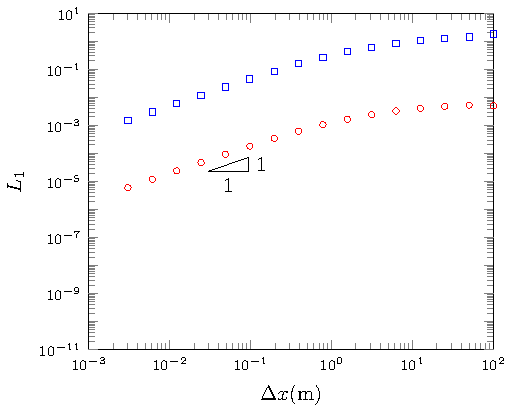
\includegraphics[width=7.0cm]{./results/soliton/con/sto1-figure0.pdf}}
\subfigure[][]{\label{fig:solitoncono2}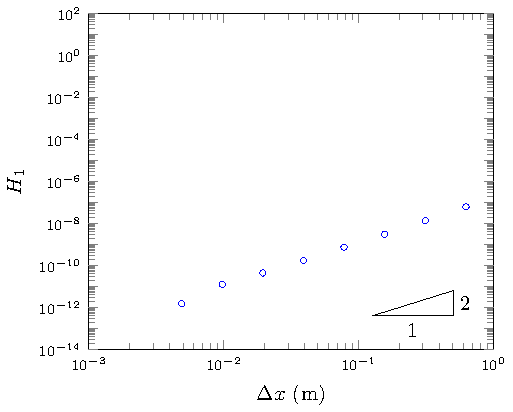
\includegraphics[width=7.0cm]{./results/soliton/con/sto2-figure0.pdf}}
\subfigure[][]{\label{fig:solitoncono3}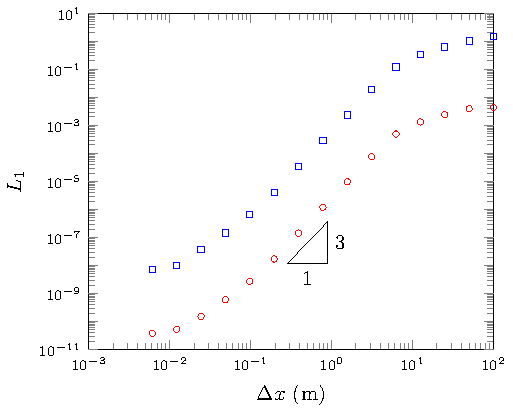
\includegraphics[width=7.0cm]{./results/soliton/con/sto3-figure0.pdf}}
\caption{Convergence of relative error using L1 norm for analytic soliton solution for both $h$ ($\circ$) and $u$ ($\diamond$) for first (a), second (b) and third (c) order schemes.}
\label{fig:solitoncon}
\end{figure}
\begin{figure}[htb]
\centering
\subfigure[][]{\label{fig:solitoneo1h}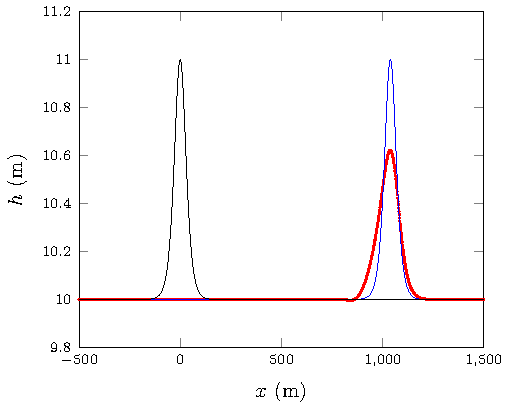
\includegraphics[width=7.0cm]{./results/soliton/ex/newo1-figure0.pdf}}
\subfigure[][]{\label{fig:solitoneo1u}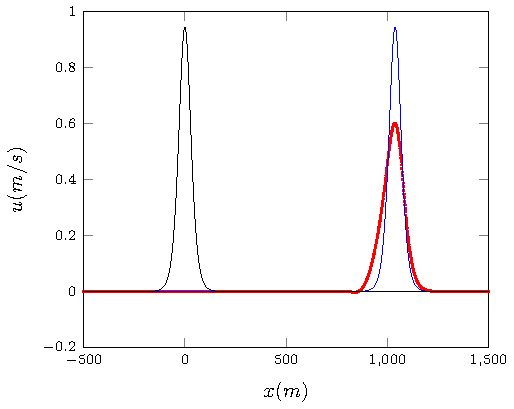
\includegraphics[width=7.0cm]{./results/soliton/ex/newo1u-figure0.pdf}}
\caption{Plotted example soliton simulation for first-order scheme ($\circ$) with $dx = 1.5625m$ against the analytic solution of \eqref{eq:sol} (\---) with black and blue for $t =0s$ and $t=100s$ respectively.}
\label{fig:solitoneo1}
\end{figure}
\begin{figure}[htb]
\centering
\subfigure[][]{\label{fig:solitoneo2h}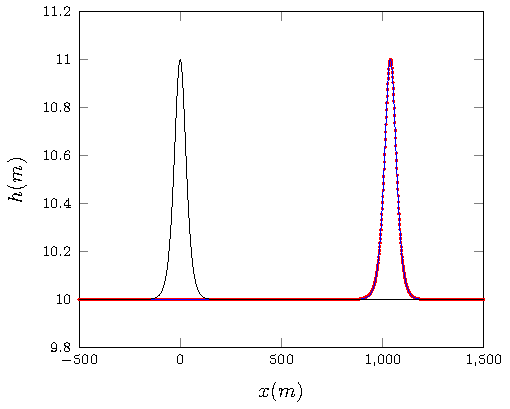
\includegraphics[width=7.0cm]{./results/soliton/ex/newo2-figure0.pdf}}
\subfigure[][]{\label{fig:solitoneo2u}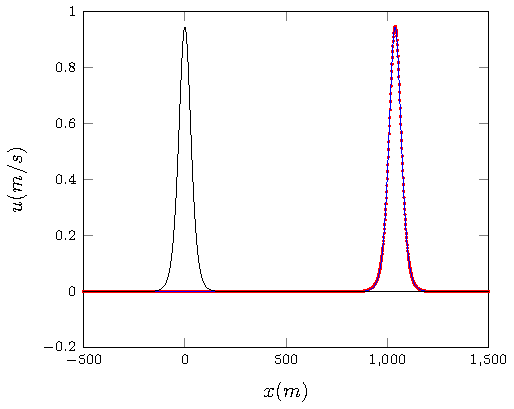
\includegraphics[width=7.0cm]{./results/soliton/ex/newo2u-figure0.pdf}}
\caption{Plotted example soliton simulation for second-order scheme ($\circ$) with $dx = 1.5625m$ against the analytic solution of \eqref{eq:sol} (\---) with black and blue for $t =0s$ and $t=100s$ respectively.}
\label{fig:solitoneo2}
\end{figure}
\begin{figure}[htb]
\centering
\subfigure[][]{\label{fig:solitoneo3h}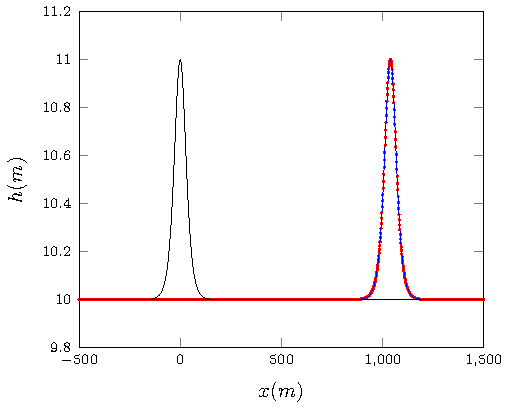
\includegraphics[width=7.0cm]{./results/soliton/ex/newo3-figure0.pdf}}
\subfigure[][]{\label{fig:solitoneo3u}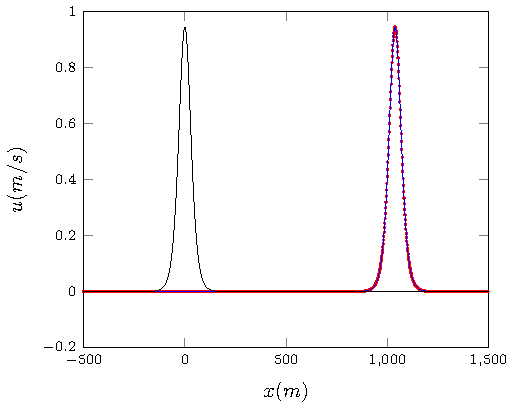
\includegraphics[width=7.0cm]{./results/soliton/ex/newo3u-figure0.pdf}}
\caption{Plotted example soliton simulation for third-order scheme ($\circ$) with $dx = 1.5625m$ against the analytic solution of \eqref{eq:sol} (\---) with black and blue for $t =0s$ and $t=100s$ respectively.}
\label{fig:solitoneo3}
\end{figure}
Currently there is only one family of analytic solutions to the Serre equations which are cnoidal waves \cite{Carter-Cienfuegos-2010-259}. This solution has been used to verify the order of convergence of the proposed methods in this paper, in particular for the soliton case of this family. Solitons travel without deformation and in the Serre equations they have the following form
\begin{linenomath*}
\begin{subequations}
\begin{gather}\label{eq:sol1}
h\left(x,t\right) = a_0 + a_1\text{sech}^2\left( \kappa\left(x - ct\right)\right),
\end{gather}
\begin{gather}\label{eq:sol2}
u\left(x,t\right) = c\left(1 - \dfrac{a_0}{h(x,t)} \right),
\end{gather}
\begin{gather}\label{eq:sol3}
\kappa = \dfrac{\sqrt{3a_1}}{2a_0 \sqrt{ a_0 + a_1}},
\end{gather}
\begin{gather}\label{eq:sol4}
c = \sqrt{g \left(a_0 + a_1\right)}.
\end{gather}
\end{subequations}
\label{eq:sol}
\end{linenomath*}
Where $a_0$ and $a_1$ are input parameters that determine the depth of the quiescent water and the maximum height of the soliton above that respectively. For the conducted simulation $a_0 = 10m$, $a_1 = 1m$ over an $x$ domain $\left[-500m,1500m\right]$ from time $\left[0s,100s\right]$. Where $\Delta t = \lambda \Delta x$ and $\lambda = 0.01$. For second-order $\theta = 1.2$. The example results for $\Delta x = 1.5625m$ can be seen in Figures \ref{fig:solitoneo1}-\ref{fig:solitoneo3}, while the relative error as measured by the L1-norm of the method can be seen in Figure \ref{fig:solitoncon}.

Firstly Figure \ref{fig:solitoncon} demonstrates that the schemes all have the correct order of convergence in both time and space as desired since $\Delta t = \lambda \Delta x$. Clearly this order of convergence is not over all $\Delta x$ the reason for this is when $\Delta x$ is large the actual problem is not discretised well since the cells are too large to represent the simulation properly. Hence the order of convergence there will be significantly lower, this can be seen for all sub-figures of Figure \ref{fig:solitoncon}. For Figure \ref{fig:solitoncono3} there is also a decrease in the order of convergence, this is because the third-order scheme has become accurate enough for the floating point errors to become significant, thus the behaviour of the order of convergence for all methods is as good as one can expect. 

Figures \ref{fig:solitoneo1}-\ref{fig:solitoneo3} demonstrate the superiority of the second- and third-order to the first-order method. This can also be seen in \ref{fig:solitoncon} where to get similar magnitude of the error for the first-order scheme and the higher order scheme requires a very small $\Delta x$ for the first order scheme. By inspecting the trailing edge of the soliton it can be seen that indeed as expected and supported by Figure \ref{fig:solitoncon} the third-order is better than the second-order method. With graphical inspection showing the third-order solution and the analytic solution to be identical on a relatively coarse grid with less than $500$ cells representing the actual soliton. 

Because of the added complexity of the higher order methods they do require more computational effort and hence are slower. In particular for an averaged single time step the first- and second-order method take $14\%$ and $50\%$ respectively of the time taken for a third-order method. Although the superior error does overcome this inefficiency as the $\Delta x$ become smaller. 
%--------------------------------------------------------------------------------
\subsection{Segur Labratory Experiment}\label{Laboratory_Experiments}
%--------------------------------------------------------------------------------
\subfiglabelskip=0pt
\begin{figure}[htb]
\centering
\subfigure[][]{\label{fig:Seguro1p0}\includegraphics[width=6.0cm]{./results/segurdata/o1/plotp0-figure0.pdf}}
\subfigure[][]{\label{fig:Seguro1p5}\includegraphics[width=6.0cm]{./results/segurdata/o1/plotp5-figure0.pdf}}
\subfigure[][]{\label{fig:Seguro1p10}\includegraphics[width=6.0cm]{./results/segurdata/o1/plotp10-figure0.pdf}}
\subfigure[][]{\label{fig:Seguro1p15}\includegraphics[width=6.0cm]{./results/segurdata/o1/plotp15-figure0.pdf}}
\subfigure[][]{\label{fig:Seguro1p20}\includegraphics[width=6.0cm]{./results/segurdata/o1/plotp20-figure0.pdf}}
\caption{Rectangular wave experiment for first order scheme at $\frac{x}{h_1}$ : $0$ (a), $50$ (b), $100$ (c), $150$ (d) and $200$ (e)}
\label{fig:Seguro1}
\end{figure}
%
\begin{figure}[htb]
\centering
\subfigure[][]{\label{fig:Seguro2p0}\includegraphics[width=6.0cm]{./results/segurdata/o2/plotp0-figure0.pdf}}
\subfigure[][]{\label{fig:Seguro2p5}\includegraphics[width=6.0cm]{./results/segurdata/o2/plotp5-figure0.pdf}}
\subfigure[][]{\label{fig:Seguro2p10}\includegraphics[width=6.0cm]{./results/segurdata/o2/plotp10-figure0.pdf}}
\subfigure[][]{\label{fig:Seguro2p15}\includegraphics[width=6.0cm]{./results/segurdata/o2/plotp15-figure0.pdf}}
\subfigure[][]{\label{fig:Seguro2p20}\includegraphics[width=6.0cm]{./results/segurdata/o2/plotp20-figure0.pdf}}
\caption{Rectangular wave experiment for second order scheme at $\frac{x}{h_1}$ : $0$ (a), $50$ (b), $100$ (c), $150$ (d) and $200$ (e)}
\label{fig:Seguro2}
\end{figure}
%
\begin{figure}[htb]
\centering
\subfigure[][]{\label{fig:Seguro3p0}\includegraphics[width=6.0cm]{./results/segurdata/o3/plotp0-figure0.pdf}}
\subfigure[][]{\label{fig:Seguro3p5}\includegraphics[width=6.0cm]{./results/segurdata/o3/plotp5-figure0.pdf}}
\subfigure[][]{\label{fig:Seguro3p10}\includegraphics[width=6.0cm]{./results/segurdata/o3/plotp10-figure0.pdf}}
\subfigure[][]{\label{fig:Seguro3p15}\includegraphics[width=6.0cm]{./results/segurdata/o3/plotp15-figure0.pdf}}
\subfigure[][]{\label{fig:Seguro3p20}\includegraphics[width=6.0cm]{./results/segurdata/o3/plotp20-figure0.pdf}}
\caption{Rectangular wave experiment for third order scheme at $\frac{x}{h_0}$ : $0$ (a), $50$ (b), $100$ (c), $150$ (d) and $200$ (e)}
\label{fig:Seguro3}
\end{figure}
In \cite{Hammack-Segur-1978-337} Hammack and Segur conducted an experiment that produced rectangular waves with the stroke of a $0.61m$ long piston flush with the wall of a wave tank $31.6m$ long and recorded the wave heights at certain positions over time. The quiescent water height $h_1$ was $0.1m$ while the stroke of the piston caused a depression with water suddenly $h_0 = 0.095m$ deep. To run this as a numerical simulation the reflected problem must be used, the result of this is that the simulation is reflected around the origin and $h_1 - h_0$ is doubled by changing $h_0$. Thus the domain is from $-60m$ to $60m$ and the simulation is run for $50s$ with $\Delta x = 0.01$, $\lambda = \frac{0.2}{\sqrt{g h_1}}$ and $\theta = 1.2$. The results of this simulation are displayed in figures \ref{fig:Seguro1} - \ref{fig:Seguro3}.

In this experiment the initial depression causes a right going rarefaction fan and a left going shock at least on the positive side of the axis. The shocks from both sides then reflect in the middle and so the shock and the rarefaction fan are travelling in the same direction. The leading wave in all the related figures is that rarefaction fan while the trailing dispersive waves are the result of the reflected shock.  

From all the related figures it can be seen that all models show good agreement between the arrival of the first wave and the period of all the waves. While Figure \ref{fig:Seguro1} shows the first-order model is too diffusive and thus under approximates the wave heights of the dispersive waves of the shock. While the second- and third-order methods over approximate them. This discrepancy can be explained by the Serre equations not taking into account viscous effects that diffuse the dispersive waves and so the Serre equations are actually producing an upper bound on the wave heights for fluids with viscosity. Although even without these effects these numerical methods still show good agreement with the experimental data thus validating them to correctly handle discontinuities. Additionally it demonstrates that the oscillations observed by produced numerical schemes for the Serre equation are physical.  
%--------------------------------------------------------------------------------
\subsection{Dam Break}
%--------------------------------------------------------------------------------
\begin{figure}[htb]
\begin{center}
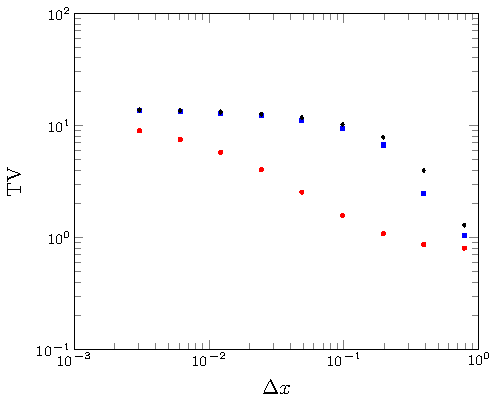
\includegraphics[width=10.0cm]{./results/dambreak/L1con/both-figure0.pdf}
\end{center}
\caption{The change in total variation (TV) over $\Delta x$ for first ($\circ$) , second ($\square$), and third ($\diamond$) order schemes.}
\label{fig:DBL1}
\end{figure}
\begin{figure}[htb]
\centering
\subfigure[][]{\label{fig:DBo1}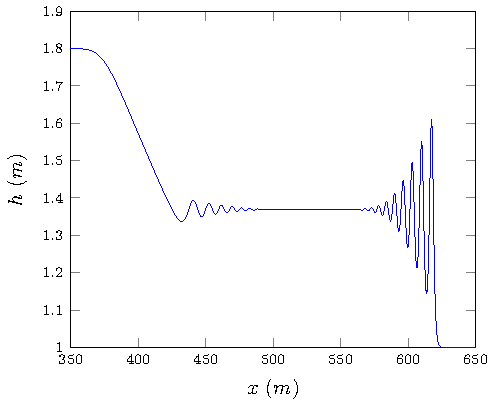
\includegraphics[width=7.0cm]{./results/dambreak/ex/o1-figure0.pdf}}
\subfigure[][]{\label{fig:DBo2}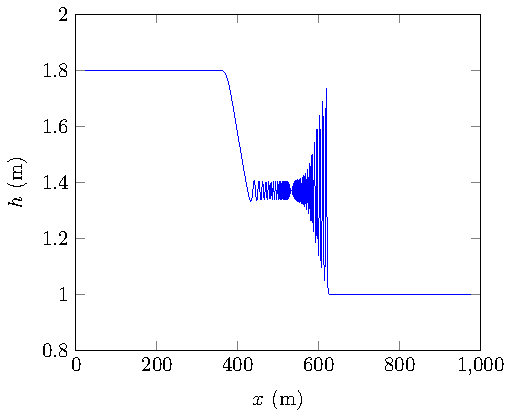
\includegraphics[width=7.0cm]{./results/dambreak/ex/o2-figure0.pdf}}
\subfigure[][]{\label{fig:DBo3}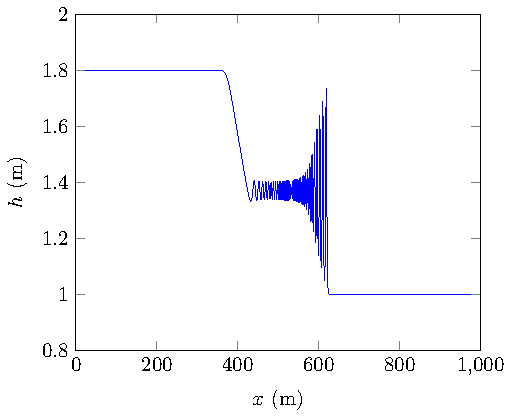
\includegraphics[width=7.0cm]{./results/dambreak/ex/o3-figure0.pdf}}
\caption{Solutions for the dam break problem for first- (a), second- (b) and third-order (c) schemes}
\label{fig:DB}
\end{figure}[]
\begin{figure}[htb]
\centering
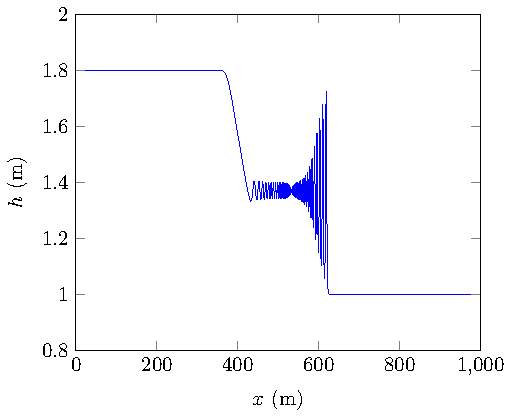
\includegraphics[width=15.0cm]{./results/dambreak/ex/o1-figure1.pdf}
\caption{Solution for the dam break problem for first-order scheme with $\Delta x = 0.00152587890625$}
\label{fig:DB1o1}
\end{figure}
The dam break problem can be defined as such
\begin{linenomath*}
\begin{gather}
h(x,0) = \left\lbrace \begin{array}{c c}
h_0 & x < x_m\\
h_1 & x \ge x_m\\
\end{array} \right. ,
\end{gather}
\begin{gather}
u(x,0) = 0.0m/s.
\end{gather}
\end{linenomath*}
For this problem the $x$ domain was $\left[0m,1000m\right]$ while the simulation was run until $t=30s$. The other values were $h_0 = 1.8m$, $h_1 = 1.0m$, $x_m = 500m$, $\lambda = 0.01$ and $\theta = 1.2$. This corresponds to sub-critical flow and was a situation demonstrated in \cite{El-etal-2006,Hank-etal-2010-2034}. An example was plotted for $\Delta x = 0.09765625m$ for all the methods described in Figure \ref{fig:DB}. To determine if the oscillations that occur in the solution indeed converge to some limit as $\Delta x \rightarrow 0$ multiple $\Delta x$ values are run and then the amount of variation in the solution measured. A common way to measure this is the total variation $TV$ \cite{LeVeque-2002} which for a vector $\boldsymbol{v}$ is given by
\begin{linenomath*}
\begin{gather}
TV(v) = \sum_{\forall i >1} |v_{i} - v_{i-1}|.
\end{gather}
\end{linenomath*}
Importantly if the solution does indeed converge to some solution then the TV must at some point plateau so that more oscillations cannot be introduced.

This is indeed the findings of the simulations that were run as can be seen by Figure \ref{fig:DBL1}. With the TV increasing as $\Delta x$ decreases at the start as the models resolve more and more dispersive waves. But as $\Delta x$ decreases further the TV plateaus and thus the oscillations are not growing without bound. Thus the scheme has not become unstable which supports further that this formulation handles shocks and the resultant dispersive waves well. Also note that as expected the higher order the method the higher TV it has at the start and the faster it plateaus and there is very good agreement between the second and third order schemes under this measure. This is surprising because as discussed in \cite{Zoppou-Roberts-1996} second-order schemes produce dissipative errors while first- and third-order schemes produce diffusive errors. What Figure \ref{fig:DBL1} and \ref{fig:DB} demonstrate is that is that the oscillations associated with dissipative errors do not make a significant impact on the profile of the dispersive waves around discontinuities. While also showing that no additional phenomena have been observed with a higher order method and so second order methods are sufficient for the Serre equations in the presence of discontinuities. 

These solutions compare very well to the findings in \cite{El-etal-2006} with both the second- and third-order schemes resolving the oscillations around the 'contact discontinuity'\cite{El-etal-2006}[] between the rarefaction fan and the shock. In \cite{Hank-etal-2010-2034} it was reported that for their first-order scheme such oscillatory behaviour was not seen but it can seen as in Figure \ref{fig:DB1o1} with $\Delta x = 0.00152587890625$.
%--------------------------------------------------------------------------------
\section{Conclusions}
\label{section:Conclusions}
%--------------------------------------------------------------------------------
A first-, second- and third-order hybrid finite difference-volume scheme were developed to solve the Serre equations in conservative form. The schemes were then tested and validated. Firstly the order of the schemes were all verified, secondly the schemes shock handling was validated by comparison with experimental data. Thirdly the behaviour of the solutions matched previous findings. Thus it can be concluded that these methods were all correct and they properly handle shocks. It was also demonstrated that for these equations second-order although not as accurate as third-order still provides a satisfactory method for reasonable $\Delta x$ unlike the first-order method which requires computationally restrictive $\Delta x$ to produce similar accuracy. This work also validates the findings in \cite{El-etal-2006},.[]  


%--------------------------------------------------------------------------------
\section{Acknowledgements}
%--------------------------------------------------------------------------------


%--------------------------------------------------------------------------------
\bibliography{Serre_ASCE}
%--------------------------------------------------------------------------------

\section{Notation}
\emph{The following symbols are used in this paper:}%\par\vspace{0.10in}
\nopagebreak
%\par
\begin{longtable}{r  @{\hspace{1em}=\hspace{1em}}  l}
$\mathcal{A}$		& Scheme to solve \eqref{eq:Gdefinition} \\
$a$					& characteristic order of free surface amplitude; \\
$B$					& characteristic order of bottom topography variation;\\
$g$					& acceleration due to gravity on earth (m/$s^2$) \\
$\mathcal{H}$		& Scheme to solve \eqref{eq:Serre_conservative_form} over a single time step \\
$H$					& characteristic water depth; \\
$h$					& water depth (m); \\
$\mathcal{L}$		& Scheme to solve \eqref{eq:Serrecon} \\
$L$					& characteristic horizontal scale; \\
$p$                 & pressure (N/m$^2$); \\
$u$                 & fluid particle velocity $x$-direction (m/s); \\
$w$                 & fluid particle velocity $z$-direction (m/s); \\
$\epsilon$			& nonlinearity parameter $a/H$ ;\\
$\xi$				& water depth from free surface (m) ;\\
$\Delta x$			& fixed resolution of $x$ ;\\
$\Delta t$			& resolution of $t$ ;\\
$\lambda$			& eigenvalues of the Jacobian ;\\
$\sigma$            & shallowness parameter $H^2/L^2$.

\end{longtable}

\section{Subscripts}
\nopagebreak
\par
\begin{tabular}{r  @{\hspace{1em}=\hspace{1em}}  l}
$i$                    & space discretisation.\\
\end{tabular}
\section{Superscripts}
\nopagebreak
\par
\begin{tabular}{r  @{\hspace{1em}=\hspace{1em}}  l}
$n$                    & time discretisation.\\
\end{tabular}
\section{accents}
\nopagebreak
\par
\begin{tabular}{r  @{\hspace{1em}=\hspace{1em}}  l}
$\bar{q}$                    &  quantity $q$ averaged over the depth of water\\
$\bar{q}$                    &  quantity $q$ averaged over a $\Delta x$ length interval of space [only make sense given a $x$ position to center the interval]\\
\end{tabular}

\end{document}
